\section{Theorie}
\label{sec:Theorie}

Zwei schwingende Systeme nennt man dann gekoppelt, wenn sie aufeinander eine Rückwirkung ausüben. 
Die Kopplung zweier schwingungsfähiger Systeme kann mithilfe äußerer Anregungen zur Energieübertragung gebracht werden, 
welche sich in Form von Resonanzeffekten erkennbar macht.\\
\\
Als ein gekoppeltes Schwingsystem sind zwei durch eine Feder verbundene Fadenpendel schwer zu untersuchen.
Es wird daher auf elektrische Schwingkreise zurückgegriffen, da Frequenz und Amplitude dabei leichter zu bestimmen sind.

\subsection {Verhalten kapazitiv gekoppelter Schwingkreise}

Es werden zwei identische Schwingkreise betrachtet, die durch eine Kapazität $C_\text{K}$ miteinander verbunden sind.

\begin{figure} 
    \centering
    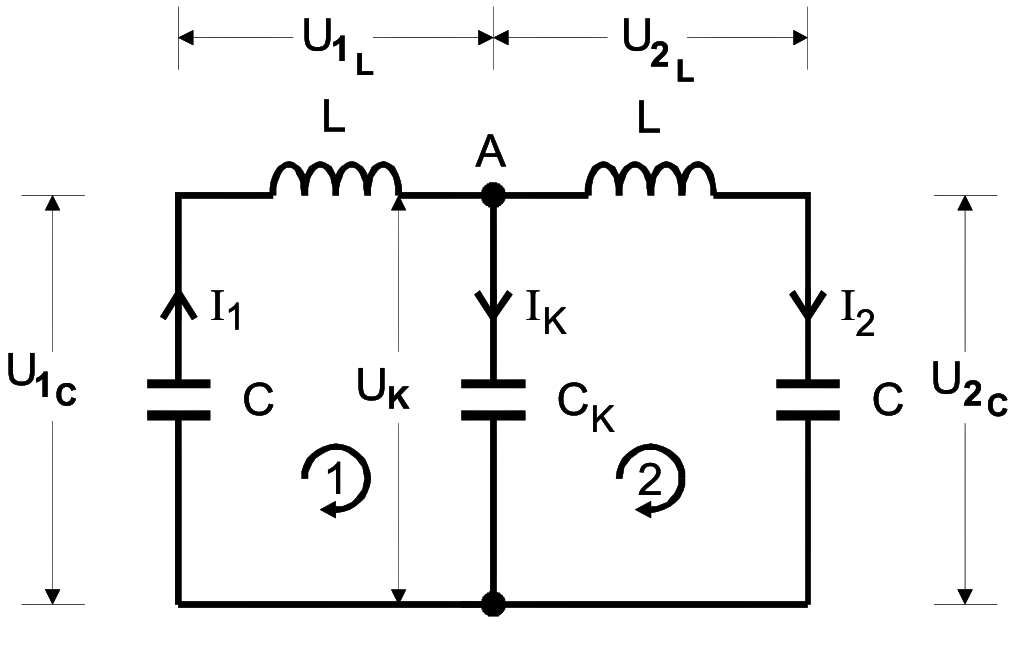
\includegraphics[width=10cm] {pictures/prinzipschaltbild.png}  
    \caption{Schaltung kapazitiv gekoppelter Schwingkreise. \cite{v355}}
    \label{fig:prinzipschaltbild}
\end{figure} 

Mithilfe der \textit{Kirchhoffschen Gesetze}, welche den Zusammenhang zwischen mehreren elektrischen Strömen und Spannungen 
beschreiben, ergibt sich im Knotenpunkt A
\begin{equation}
    I_{1} = I_\text{K} + I_{2} \,.
\end{equation}

Für Masche 1 und 2 ergibt sich
\begin{equation}
    U_{{1,2}_{C}} + U_{{1,2}_\text{L}} + U_\text{K} = 0 \,.
\end{equation}

In dieses Gleichungssystem werden die Beziehungen
\begin{equation} 
    U_{C} = \frac{1}{C} \dif{t} \int I \quad\text{und}\quad U_\text{L} = L \dot{I} \quad\text{ein.}
\end{equation}

eingesetzt. Damit ergeben sich für die beiden Maschen mit Differentiation nach $t$ die Differentialgleichungen
\begin{align}  
    L {\dot{I}}_{1} + \frac{1}{C} I_{1} + \frac{1}{C_\text{K}} (I_{1} - I_{2})  &= 0 \label{eq:dgl_1} \\
    L {\dot{I}}_{2} + \frac{1}{C} I_{2} + \frac{1}{C_\text{K}} (I_{1} - I_{2})  &= 0 \label{eq:dgl_2} \,.
\end{align}

Addition und Subtraktion der Gleichungen (\ref{eq:dgl_1}) und (\ref{eq:dgl_2}) ergibt die entkoppelten 
Differentialgleichungen für die neuen Variablen ($I_{1}+I_{2}$) und ($I_{1}-I_{2}$)
\begin{align} 
    L \frac {\dif{^2}} {\dif{t^2}} (I_{1} + I_{2}) + \frac{1}{C} (I_{1} + I_{2})  &= 0 \label{eq:dgl_1_entk} \\
    L \frac {\dif{^2}} {\dif{t^2}} (I_{1} - I_{2}) + \left( \frac{1}{C} + \frac{2}{C_\text{K}} \right) (I_{1} - I_{2})  &= 0 \label{eq:dgl_2_entk} \,.
\end{align}

Diese werden durch
\begin{align}
    (I_{1} + I_{2})(t) &= (I_{1,0} + I_{2,0}) \cos(I_{1} + I_{2}) \label{eq:dgl_1_sumsol} \\
    (I_{1} - I_{2})(t) &= (I_{1,0} - I_{2,0}) \cos \left( \frac {t} {{\sqrt [] {L \left( \frac{1}{C} + \frac{2}{C_\text{K}} \right)^{-1} }}} \right) \label{eq:dgl_2_sumsol}
\end{align}

gelöst. Durch erneute Addition und Subtraktion von (\ref{eq:dgl_1_sumsol}) und (\ref{eq:dgl_2_sumsol}) ergeben sich die Lösungen 
der ursprünglichen Ströme $I_{1}$ und $I_{2}$
\begin{align}
    I_{1}(t) &= \frac{1}{2} (I_{1,0} + I_{2,0}) \cos(2 \pi \nu^+ t)  +  \frac{1}{2} (I_{1,0} - I_{2,0}) \cos(2 \pi \nu^- t) \label{eq:dgl_1_sol} \\
    I_{2}(t) &= \frac{1}{2} (I_{1,0} + I_{2,0}) \cos(2 \pi \nu^+ t)  -  \frac{1}{2} (I_{1,0} - I_{2,0}) \cos(2 \pi \nu^- t) \label{eq:dgl_2_sol} \,,
\end{align}

wobei 
\begin{align}
    \nu^+ &= \frac {1} {2 \pi \sqrt[]{LC}} & \mbox{\centering und} && \nu^- = \frac {t} {2 \pi \sqrt [] {L \left( \frac{1}{C} + \frac{2}{C_\text{K}} \right)^{-1} }}
\end{align}

die Schwingungsfrequenzen von (\ref{eq:dgl_1_sumsol}) und (\ref{eq:dgl_2_sumsol}) darstellen. \\
\\
Sind zu Beginn die Amplituden beider Schwingkreise gleich groß ($I_{1,0} = I_{2,0}$), so entfallen bei (\ref{eq:dgl_1_sol}) und (\ref{eq:dgl_2_sol})
die jeweils letzten Terme. In diesem Fall schwingen die beiden Schwingkreise gleichphasig mit der Schwingunsfrequenz $\nu^+$, am
Koppelkondensator $C_\text{K}$ leigt dabei nie eine Spannung an. Bei gegengleichen Amplituden ($I_{1,0} = -I_{2,0}$) schwingen die Schwingkreise gegenphasig
mit der erhöhten Schwingunsfrequenz $\nu^-$ und die Spannung an $C_\text{K}$ wird maximal. Diese beiden Schwingungstypen werden \textit{Fundamentalschwingungen} genannt. \\
\\
Wird hingegen nur einer der beiden Schwingkreise ausgelenkt ($I_{1,0} \neq 0, I_{2,0} = 0$), so ergeben sich Schwebungen.
\begin{align}
    I_{1}(t) &= I_{1,0} \cos(\pi (\nu^+ + \nu^-) t) \cos(\pi (\nu^+ - \nu^-) t) \label{eq:dgl_1_sol_schweb} \\
    I_{2}(t) &= I_{1,0} \sin(\pi (\nu^+ + \nu^-) t) \sin(\pi (\nu^+ - \nu^-) t) \label{eq:dgl_2_sol_schweb} 
\end{align}

Der Verlauf der Ströme $I_{1}(t)$ und $I_{2}(t)$ werden in Abbildung (\ref{fig:schwebung}) dargestellt.
\begin{figure} 
    \centering
    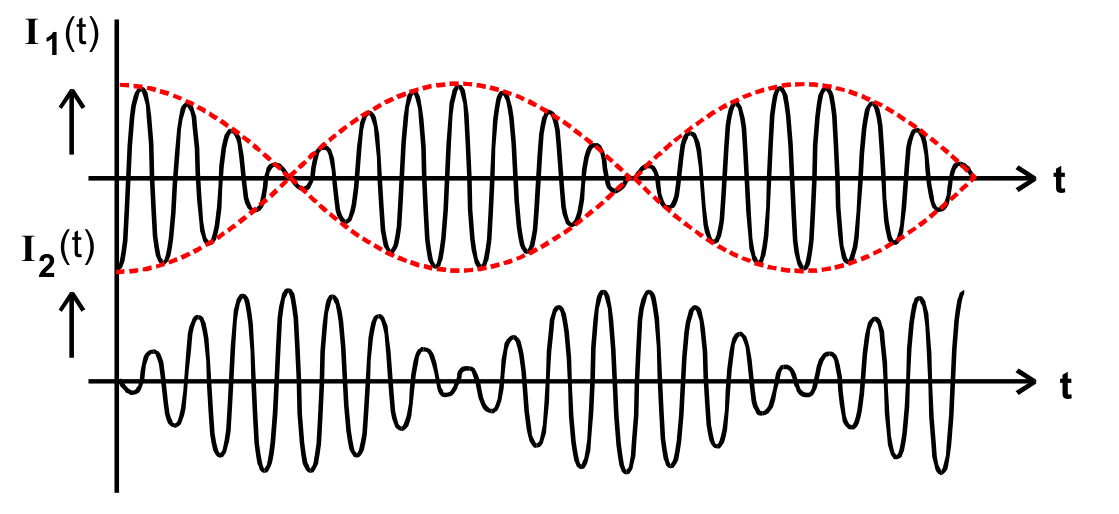
\includegraphics[width=10cm] {pictures/schwebung.png} 
    \caption{Zeitlicher Verlauf der Ströme im Falle einer Schwebung. \cite{v355}}
    \label{fig:schwebung}
\end{figure} 

Bei diesen Anfangsbedingungen wird die Energie des ausgelenkten Schwingkreises auf den ruhenden übertragen, was eine gekoppelte Schwingung zur Folge hat.
Die Amplitude der Schwingungsfrequenz ändert sich mit der \textit{Schwebungungsfrequenz} 
\begin{align}
    \nu_\text{Schwebung} &= \nu^- - \nu^+ \., \\
    \intertext{während das System mit der Schwingungsfrequenz}
    \nu_\text{Schwingung} &= \frac{1}{2} \left( \nu^+ + \nu^- \right) \approx \nu^+ 
\end{align}
schwingt.


\subsection {Abhängigkeit des Stromes von der Frequenz}

Werden die Schwingkreise durch eine von außen angelegte Sinusspannung angeregt (siehe Abblildung \ref{fig:sinusspannung}), \\
\begin{figure} 
    \centering
    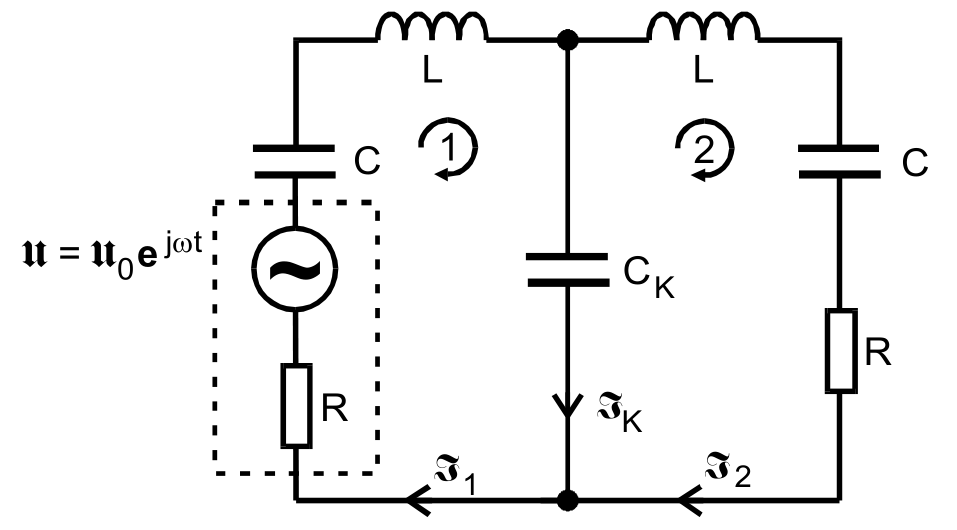
\includegraphics[width=10cm] {pictures/sinusspannung.png} 
    \caption{Schwingkreise mit Sinusgenerator. \cite{v355}}
    \label{fig:sinusspannung}
\end{figure} 

so ergeben sich mithilfe der \textit{Kirchhoffschen Maschenregel} die Gleichungen
\begin{align}
    U &= (z_{C} + z_\text{L} + z_{C_\text{K}} + z_{R}) I_{1} - z_{C_\text{K}} I_{2} \label{eq:sin_masche_1} \\
    0 &= (z_{C} + z_\text{L} + z_{C_\text{K}} + z_{R}) I_{2} - z_{C_\text{K}} I_{1} \label{eq:sin_masche_2} 
\end{align}

mit den Impedanzen
\begin{align} 
    z_{C} &= \frac{1}{i \omega C} & z_\text{L} = i \omega L  && z_{R} = R \.,
\end{align}

Nach Elimination von $I_{1}$ folgt für $I_{2}$ 
\begin{align}
    I_{2} &=U \frac{\frac{1}{i \omega C_\text{K}}}{\left(i \omega L+\frac{1}{i \omega C}+\frac{1}{i \omega C_\text{K}}+R\right)^{2}+\frac{1}{\omega^{2} C_\text{K}^{2}}} \label{eq:strom2} \\
    \Rightarrow\left|I_{2}\right| &=\lvert U\rvert \frac{1}{\sqrt{4 \omega^{2} C_\text{K}^{2} R^{2} Z(\omega)^{2}+\left(\frac{1}{\omega C_\text{K}}-\omega C_\text{K} Z(\omega)^{2}+\omega R^{2} C_\text{K}\right)^{2}}} \label{eq:betrag_strom2}     
\end{align}

mit
\begin{align}
    Z(\omega)=\omega L-\frac{1}{\omega\left(\frac{1}{C}+\frac{1}{C_\text{K}}\right)^{-1}}
\end{align}

Der Strom $I_{2}$ nimmt für $\nu^+$ und $\nu^-$ seine Maxima an:
\begin{align}
    \left|I_{2}\left(\omega^{+}\right)\right| &= \frac{1}{R \sqrt{4+\frac{R^{2} C_\text{K}^{2}}{L C}}} \label{eq:strom2_omegaplus}\\
    \left|I_{2}\left(\omega^{-}\right)\right| &= \frac{1}{R \sqrt{4+\frac{R^{2} C_\text{K}^{2}}{L C}\left(1+\frac{C}{C_\text{K}}\right)}} \label{eq:strom2_omegaminus}
\end{align}
